\section{CLocation\-Monitor$<$ T $>$  Class Template Reference}
\label{classCLocationMonitor}\index{CLocationMonitor@{CLocation\-Monitor}}
{\tt \#include $<$CLocation\-Monitor.h$>$}

Inheritance diagram for CLocation\-Monitor$<$ T $>$::\begin{figure}[H]
\begin{center}
\leavevmode
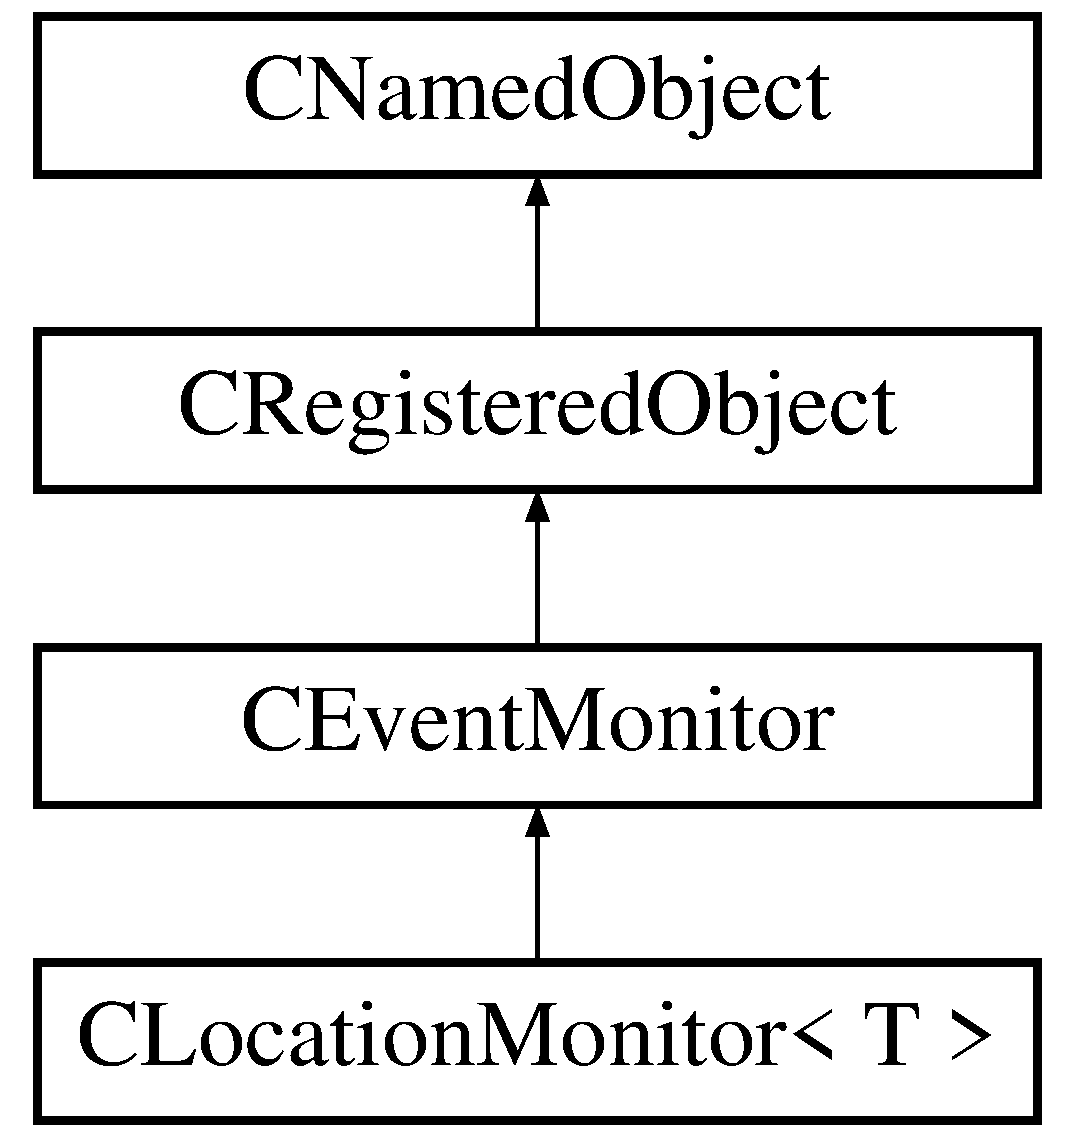
\includegraphics[height=4cm]{classCLocationMonitor}
\end{center}
\end{figure}
\subsection*{Public Methods}
\begin{CompactItemize}
\item 
{\bf CLocation\-Monitor} (volatile T $\ast$am\_\-p\-TLocation, {\bf CPointer\-Predicate}$<$ T $>$ $\ast$am\_\-Predicate, bool am\_\-f\-Timed\-Wait=true)
\item 
{\bf CLocation\-Monitor} (const string \&r\-Name, volatile T $\ast$am\_\-p\-TLocation, {\bf CPointer\-Predicate}$<$ T $>$ $\ast$am\_\-Predicate, bool am\_\-f\-Timed\-Wait=true)
\item 
{\bf CLocation\-Monitor} (const char $\ast$p\-Name, volatile T $\ast$am\_\-p\-TLocation, {\bf CPointer\-Predicate}$<$ T $>$ $\ast$am\_\-Predicate, bool am\_\-f\-Timed\-Wait=true)
\item 
{\bf $\sim$CLocation\-Monitor} ()
\item 
int {\bf operator==} (const CLocation\-Monitor$<$ T $>$ \&a\-CLocation\-Monitor) const
\item 
volatile T $\ast$ {\bf get\-Location} () const
\item 
{\bf CPointer\-Predicate}$<$ T $>$ {\bf get\-Predicate} () const
\item 
virtual {\bf CEvent\-Monitor::result} {\bf operator()} ()
\item 
void {\bf Change\-Location} (T $\ast$p\-New\-Location)
\item 
void {\bf Change\-Predicate} ({\bf CPointer\-Predicate}$<$ T $>$ $\ast$newloc)
\item 
T {\bf get\-Contents} () const
\item 
virtual string {\bf Describe\-Self} ()
\end{CompactItemize}
\subsection*{Protected Methods}
\begin{CompactItemize}
\item 
void {\bf set\-Location} (volatile T $\ast$am\_\-p\-TLocation)
\item 
void {\bf set\-Predicate} ({\bf CPointer\-Predicate}$<$ T $>$ \&am\_\-Predicate)
\end{CompactItemize}
\subsection*{Private Methods}
\begin{CompactItemize}
\item 
{\bf CLocation\-Monitor} (const CLocation\-Monitor$<$ T $>$ \&a\-CLocation\-Monitor)
\item 
CLocation\-Monitor$<$ T $>$ {\bf operator=} (const CLocation\-Monitor$<$ T $>$ \&a\-CLocation\-Monitor)
\end{CompactItemize}
\subsection*{Private Attributes}
\begin{CompactItemize}
\item 
volatile T $\ast$ {\bf m\_\-p\-TLocation}
\item 
{\bf CPointer\-Predicate}$<$ T $>$ $\ast$ {\bf m\_\-Predicate}
\end{CompactItemize}


\subsection{Detailed Description}
\subsubsection*{template$<$typename T$>$ class CLocation\-Monitor$<$ T $>$}

Encapsulates a location monitor.  The location monitor watches a volatile memory location  to satisfy some predicate function object. Predicates are objects from classes which implement: bool operator()(T value) T is a templated variable of the class. Such objects are function objects. The  Event is fired when the predicate returns TRUE. 



Definition at line 335 of file CLocation\-Monitor.h.

\subsection{Constructor \& Destructor Documentation}
\index{CLocationMonitor@{CLocation\-Monitor}!CLocationMonitor@{CLocationMonitor}}
\index{CLocationMonitor@{CLocationMonitor}!CLocationMonitor@{CLocation\-Monitor}}
\subsubsection{\setlength{\rightskip}{0pt plus 5cm}template$<$typename T$>$ CLocation\-Monitor$<$ T $>$::CLocation\-Monitor (volatile T $\ast$ {\em am\_\-p\-TLocation}, {\bf CPointer\-Predicate}$<$ T $>$ $\ast$ {\em am\_\-Predicate}, bool {\em am\_\-f\-Timed\-Wait} = true)\hspace{0.3cm}{\tt  [inline]}}\label{classCLocationMonitor_a0}


associated predicate \index{CLocationMonitor@{CLocation\-Monitor}!CLocationMonitor@{CLocationMonitor}}
\index{CLocationMonitor@{CLocationMonitor}!CLocationMonitor@{CLocation\-Monitor}}
\subsubsection{\setlength{\rightskip}{0pt plus 5cm}template$<$typename T$>$ CLocation\-Monitor$<$ T $>$::CLocation\-Monitor (const string \& {\em r\-Name}, volatile T $\ast$ {\em am\_\-p\-TLocation}, {\bf CPointer\-Predicate}$<$ T $>$ $\ast$ {\em am\_\-Predicate}, bool {\em am\_\-f\-Timed\-Wait} = true)\hspace{0.3cm}{\tt  [inline]}}\label{classCLocationMonitor_a1}


\index{CLocationMonitor@{CLocation\-Monitor}!CLocationMonitor@{CLocationMonitor}}
\index{CLocationMonitor@{CLocationMonitor}!CLocationMonitor@{CLocation\-Monitor}}
\subsubsection{\setlength{\rightskip}{0pt plus 5cm}template$<$typename T$>$ CLocation\-Monitor$<$ T $>$::CLocation\-Monitor (const char $\ast$ {\em p\-Name}, volatile T $\ast$ {\em am\_\-p\-TLocation}, {\bf CPointer\-Predicate}$<$ T $>$ $\ast$ {\em am\_\-Predicate}, bool {\em am\_\-f\-Timed\-Wait} = true)\hspace{0.3cm}{\tt  [inline]}}\label{classCLocationMonitor_a2}


\index{CLocationMonitor@{CLocation\-Monitor}!~CLocationMonitor@{$\sim$CLocationMonitor}}
\index{~CLocationMonitor@{$\sim$CLocationMonitor}!CLocationMonitor@{CLocation\-Monitor}}
\subsubsection{\setlength{\rightskip}{0pt plus 5cm}template$<$typename T$>$ CLocation\-Monitor$<$ T $>$::$\sim$CLocation\-Monitor ()\hspace{0.3cm}{\tt  [inline]}}\label{classCLocationMonitor_a3}


\index{CLocationMonitor@{CLocation\-Monitor}!CLocationMonitor@{CLocationMonitor}}
\index{CLocationMonitor@{CLocationMonitor}!CLocationMonitor@{CLocation\-Monitor}}
\subsubsection{\setlength{\rightskip}{0pt plus 5cm}template$<$typename T$>$ CLocation\-Monitor$<$ T $>$::CLocation\-Monitor (const CLocation\-Monitor$<$ T $>$ \& {\em a\-CLocation\-Monitor})\hspace{0.3cm}{\tt  [private]}}\label{classCLocationMonitor_c0}




\subsection{Member Function Documentation}
\index{CLocationMonitor@{CLocation\-Monitor}!ChangeLocation@{ChangeLocation}}
\index{ChangeLocation@{ChangeLocation}!CLocationMonitor@{CLocation\-Monitor}}
\subsubsection{\setlength{\rightskip}{0pt plus 5cm}template$<$typename T$>$ void CLocation\-Monitor$<$ T $>$::Change\-Location (T $\ast$ {\em p\-New\-Location})}\label{classCLocationMonitor_a8}


Operation Type: Mutator

Purpose: Changes the location monitored. 

Definition at line 354 of file CLocation\-Monitor.cpp.

References CLocation\-Monitor$<$ T $>$::m\_\-p\-TLocation.\index{CLocationMonitor@{CLocation\-Monitor}!ChangePredicate@{ChangePredicate}}
\index{ChangePredicate@{ChangePredicate}!CLocationMonitor@{CLocation\-Monitor}}
\subsubsection{\setlength{\rightskip}{0pt plus 5cm}template$<$typename T$>$ void CLocation\-Monitor$<$ T $>$::Change\-Predicate ({\bf CPointer\-Predicate}$<$ T $>$ $\ast$ {\em new\-Loc})}\label{classCLocationMonitor_a9}


Operation Type: Mutator

Purpose: Associates a new predicate with the  location monitor. 

Definition at line 371 of file CLocation\-Monitor.cpp.

References CLocation\-Monitor$<$ T $>$::m\_\-Predicate.\index{CLocationMonitor@{CLocation\-Monitor}!DescribeSelf@{DescribeSelf}}
\index{DescribeSelf@{DescribeSelf}!CLocationMonitor@{CLocation\-Monitor}}
\subsubsection{\setlength{\rightskip}{0pt plus 5cm}template$<$typename T$>$ string CLocation\-Monitor$<$ T $>$::Describe\-Self ()\hspace{0.3cm}{\tt  [virtual]}}\label{classCLocationMonitor_a11}


Operation Type: Selector

Purpose: Returns a string which describes the monitor. Inlcudes: 1. {\bf CEvent\-Monitor::Describe\-Self} {\rm (p.\,\pageref{classCNamedObject_a8})} 2. Dumps of the pointer value, 3. m\_\-Predicate-$>${\bf Describe\-Self}() {\rm (p.\,\pageref{classCLocationMonitor_a11})} 

Reimplemented from {\bf CNamed\-Object} {\rm (p.\,\pageref{classCNamedObject_a8})}.

Definition at line 390 of file CLocation\-Monitor.cpp.

References CNamed\-Object::Describe\-Self(), CLocation\-Monitor$<$ T $>$::m\_\-Predicate, and CLocation\-Monitor$<$ T $>$::m\_\-p\-TLocation.\index{CLocationMonitor@{CLocation\-Monitor}!getContents@{getContents}}
\index{getContents@{getContents}!CLocationMonitor@{CLocation\-Monitor}}
\subsubsection{\setlength{\rightskip}{0pt plus 5cm}template$<$typename T$>$ T CLocation\-Monitor$<$ T $>$::get\-Contents () const\hspace{0.3cm}{\tt  [inline]}}\label{classCLocationMonitor_a10}




Definition at line 419 of file CLocation\-Monitor.h.\index{CLocationMonitor@{CLocation\-Monitor}!getLocation@{getLocation}}
\index{getLocation@{getLocation}!CLocationMonitor@{CLocation\-Monitor}}
\subsubsection{\setlength{\rightskip}{0pt plus 5cm}template$<$typename T$>$ volatile T$\ast$ CLocation\-Monitor$<$ T $>$::get\-Location () const\hspace{0.3cm}{\tt  [inline]}}\label{classCLocationMonitor_a5}




Definition at line 390 of file CLocation\-Monitor.h.

References CLocation\-Monitor$<$ T $>$::m\_\-p\-TLocation.

Referenced by CLocation\-Event$<$ T $>$::get\-Pointer(), and CLocation\-Reactor$<$ T $>$::On\-Event().\index{CLocationMonitor@{CLocation\-Monitor}!getPredicate@{getPredicate}}
\index{getPredicate@{getPredicate}!CLocationMonitor@{CLocation\-Monitor}}
\subsubsection{\setlength{\rightskip}{0pt plus 5cm}template$<$typename T$>$ {\bf CPointer\-Predicate}$<$T$>$ CLocation\-Monitor$<$ T $>$::get\-Predicate () const\hspace{0.3cm}{\tt  [inline]}}\label{classCLocationMonitor_a6}




Definition at line 395 of file CLocation\-Monitor.h.\index{CLocationMonitor@{CLocation\-Monitor}!operator()@{operator()}}
\index{operator()@{operator()}!CLocationMonitor@{CLocation\-Monitor}}
\subsubsection{\setlength{\rightskip}{0pt plus 5cm}template$<$typename T$>$ {\bf CEvent\-Monitor::result} CLocation\-Monitor$<$ T $>$::operator() ()\hspace{0.3cm}{\tt  [virtual]}}\label{classCLocationMonitor_a7}


Operation Type: Override behavior

Purpose: Reads the current value of the location and passes it to the predicate. Returns: 1. Occured - if the predicate returned TRUE 2. Timed\-Out - if the wait time for this event timedout. 3. Error - If the predicate threw an exception. 

Implements {\bf CEvent\-Monitor} {\rm (p.\,\pageref{classCEventMonitor_a7})}.

Definition at line 315 of file CLocation\-Monitor.cpp.

References CEvent\-Monitor::Error, CEvent\-Monitor::get\-Timeout(), INCREMENTS, CLocation\-Monitor$<$ T $>$::m\_\-Predicate, CEvent\-Monitor::Occurred, and CEvent\-Monitor::Timed\-Out.\index{CLocationMonitor@{CLocation\-Monitor}!operator=@{operator=}}
\index{operator=@{operator=}!CLocationMonitor@{CLocation\-Monitor}}
\subsubsection{\setlength{\rightskip}{0pt plus 5cm}template$<$typename T$>$ CLocation\-Monitor$<$T$>$ CLocation\-Monitor$<$ T $>$::operator= (const CLocation\-Monitor$<$ T $>$ \& {\em a\-CLocation\-Monitor})\hspace{0.3cm}{\tt  [private]}}\label{classCLocationMonitor_c1}


\index{CLocationMonitor@{CLocation\-Monitor}!operator==@{operator==}}
\index{operator==@{operator==}!CLocationMonitor@{CLocation\-Monitor}}
\subsubsection{\setlength{\rightskip}{0pt plus 5cm}template$<$typename T$>$ int CLocation\-Monitor$<$ T $>$::operator== (const CLocation\-Monitor$<$ T $>$ \& {\em a\-CLocation\-Monitor}) const\hspace{0.3cm}{\tt  [inline]}}\label{classCLocationMonitor_a4}




Definition at line 371 of file CLocation\-Monitor.h.

References CLocation\-Monitor$<$ T $>$::m\_\-Predicate, CLocation\-Monitor$<$ T $>$::m\_\-p\-TLocation, and CEvent\-Monitor::operator==().\index{CLocationMonitor@{CLocation\-Monitor}!setLocation@{setLocation}}
\index{setLocation@{setLocation}!CLocationMonitor@{CLocation\-Monitor}}
\subsubsection{\setlength{\rightskip}{0pt plus 5cm}template$<$typename T$>$ void CLocation\-Monitor$<$ T $>$::set\-Location (volatile T $\ast$ {\em am\_\-p\-TLocation})\hspace{0.3cm}{\tt  [inline, protected]}}\label{classCLocationMonitor_b0}




Definition at line 403 of file CLocation\-Monitor.h.

References CLocation\-Monitor$<$ T $>$::m\_\-p\-TLocation.\index{CLocationMonitor@{CLocation\-Monitor}!setPredicate@{setPredicate}}
\index{setPredicate@{setPredicate}!CLocationMonitor@{CLocation\-Monitor}}
\subsubsection{\setlength{\rightskip}{0pt plus 5cm}template$<$typename T$>$ void CLocation\-Monitor$<$ T $>$::set\-Predicate ({\bf CPointer\-Predicate}$<$ T $>$ \& {\em am\_\-Predicate})\hspace{0.3cm}{\tt  [inline, protected]}}\label{classCLocationMonitor_b1}




Definition at line 408 of file CLocation\-Monitor.h.

\subsection{Member Data Documentation}
\index{CLocationMonitor@{CLocation\-Monitor}!m_Predicate@{m\_\-Predicate}}
\index{m_Predicate@{m\_\-Predicate}!CLocationMonitor@{CLocation\-Monitor}}
\subsubsection{\setlength{\rightskip}{0pt plus 5cm}template$<$typename T$>$ {\bf CPointer\-Predicate}$<$T$>$$\ast$ CLocation\-Monitor$<$ T $>$::m\_\-Predicate\hspace{0.3cm}{\tt  [private]}}\label{classCLocationMonitor_o1}


Location monitored 

Definition at line 338 of file CLocation\-Monitor.h.

Referenced by CLocation\-Monitor$<$ T $>$::Change\-Predicate(), CLocation\-Monitor$<$ T $>$::Describe\-Self(), CLocation\-Monitor$<$ T $>$::operator()(), and CLocation\-Monitor$<$ T $>$::operator==().\index{CLocationMonitor@{CLocation\-Monitor}!m_pTLocation@{m\_\-pTLocation}}
\index{m_pTLocation@{m\_\-pTLocation}!CLocationMonitor@{CLocation\-Monitor}}
\subsubsection{\setlength{\rightskip}{0pt plus 5cm}template$<$typename T$>$ volatile T$\ast$ CLocation\-Monitor$<$ T $>$::m\_\-p\-TLocation\hspace{0.3cm}{\tt  [private]}}\label{classCLocationMonitor_o0}




Definition at line 337 of file CLocation\-Monitor.h.

Referenced by CLocation\-Monitor$<$ T $>$::Change\-Location(), CLocation\-Monitor$<$ T $>$::Describe\-Self(), CLocation\-Monitor$<$ T $>$::get\-Location(), CLocation\-Monitor$<$ T $>$::operator==(), and CLocation\-Monitor$<$ T $>$::set\-Location().

The documentation for this class was generated from the following files:\begin{CompactItemize}
\item 
{\bf CLocation\-Monitor.h}\item 
{\bf CLocation\-Monitor.cpp}\end{CompactItemize}
